\documentclass[11pt]{article}
%% Stylefile to load PR Letters template
%\usepackage{prletters}
\usepackage{framed,multirow}
\usepackage{algorithm}
\usepackage{algpseudocode}
%% The amssymb package provides various useful mathematical symbols
\usepackage{amssymb}
\usepackage{latexsym}
\usepackage{url}
\usepackage{amsfonts} 
\usepackage{amsmath}
\usepackage{amsthm}
\usepackage{pifont}
\usepackage{natbib}
\usepackage{geometry}
\usepackage{graphicx}
\usepackage{color} 
 
\newcommand{\subfigimg}[3][,]{%
  \setbox1=\hbox{\includegraphics[#1]{#3}}% Store image in box
  \leavevmode\rlap{\usebox1}% Print image
  \rlap{\hspace*{12pt}\raisebox{\dimexpr\ht1-0\baselineskip}{#2}}% Print label
  \phantom{\usebox1}% Insert appropriate spcing
}
%ming's package for numerical section 
\RequirePackage{lineno}
\usepackage{subfig}
%\usepackage{setspace}

\newenvironment{Table}
  {\par\bigskip\noindent\minipage{\columnwidth}\centering}
  {\endminipage\par\bigskip}
	
%flowchart
\usepackage{tikz}
\usetikzlibrary{shapes.geometric, arrows}
\tikzstyle{node} = [rectangle, rounded corners, minimum width=0.5cm, minimum height=0.5cm,text centered, draw=black, fill=white!30]
\tikzstyle{arrow} = [thick,->,>=stealth]

\newcommand{\jv}[1]{{\color{magenta}{\it #1}}}
\newcommand{\cs}[1]{{\color{blue}{\it #1}}}
\newcommand{\Linefor}[2]{%
    \State \algorithmicfor\ {#1}\ \algorithmicdo\ {#2} \algorithmicend\ \algorithmicfor%
}
\newcommand{\Lineif}[2]{%
    \State \algorithmicif\ {#1}\ \algorithmicdo\ {#2} \algorithmicend\ \algorithmicif%
}
\newcommand{\rto}{\leftarrow}
\providecommand{\mb}[1]{\boldsymbol{#1}}

\begin{document}

%\setcounter{figure}{0}
\renewcommand{\thefigure}{A\arabic{figure}}

\section{Supplementary Figures}

\begin{figure*}[htbp]
  \centering
  \begin{tabular}{@{}p{\linewidth}@{\quad}p{\linewidth}@{}}
	\centering
    \subfigimg[width=0.32\linewidth]{A}{SwissRollPower1}
    \subfigimg[width=0.32\linewidth]{B}{SwissRollNoisePower1}
    \subfigimg[width=0.32\linewidth]{C}{SwissRollOutlierPower1}
  \end{tabular}
  \caption{ Testing Power of 3D Swiss Roll versus its 2D Underlying Linear Manifold at type $1$ error level $0.05$, under the same setting as Figure 3 in the main paper.
(A) Testing Power with respect to Increasing Size of Training Data.
(B) Testing Power with respect to Increasing Noise at $n=1000$.
(C) Testing Power with respect to Growing Number of Outliers at $n=1000$. }
\label{figA1}
\end{figure*}

\begin{figure*}[htbp]
  \centering
  \begin{tabular}{@{}p{\linewidth}@{\quad}p{\linewidth}@{}}
	\centering
    \subfigimg[width=0.32\linewidth]{A}{SwissRollAcc1}
    \subfigimg[width=0.32\linewidth]{B}{SwissRollNoiseAcc1}
    \subfigimg[width=0.32\linewidth]{C}{SwissRollOutlierAcc1}
  \end{tabular}
  \caption{ Matching Ratio of 3D Swiss Roll versus its 2D Underlying Linear Manifold via CCA matching, under the same setting as Figure 3.
(A) Matching Ratio with respect to Increasing Size of Training Data.
(B) Matching Ratio with respect to Increasing Noise at $n=1000$.
(C) Matching Ratio with respect to Growing Number of Outliers at $n=1000$. }
\label{figA2}
\end{figure*}

\begin{figure*}[htbp]
  \centering
  \begin{tabular}{@{}p{\linewidth}@{\quad}p{\linewidth}@{}}
	\centering
    \subfigimg[width=0.32\linewidth]{A}{WikiTETF.png}
    \subfigimg[width=0.32\linewidth]{B}{WikiTEGE.png}
    \subfigimg[width=0.32\linewidth]{C}{WikiGEGF.png}
  \end{tabular}
  \caption{Testing Powers of Wikipedia Datasets with respect to Increasing Type $1$ Error Level.
(A) Testing Power of Wikipedia English Text versus French Text.
(B) Testing Power of Wikipedia English Text versus English Graph.
(C) Testing Power of Wikipedia English Graph versus French Graph.}
\end{figure*}

\begin{figure*}[htbp]
  \centering
	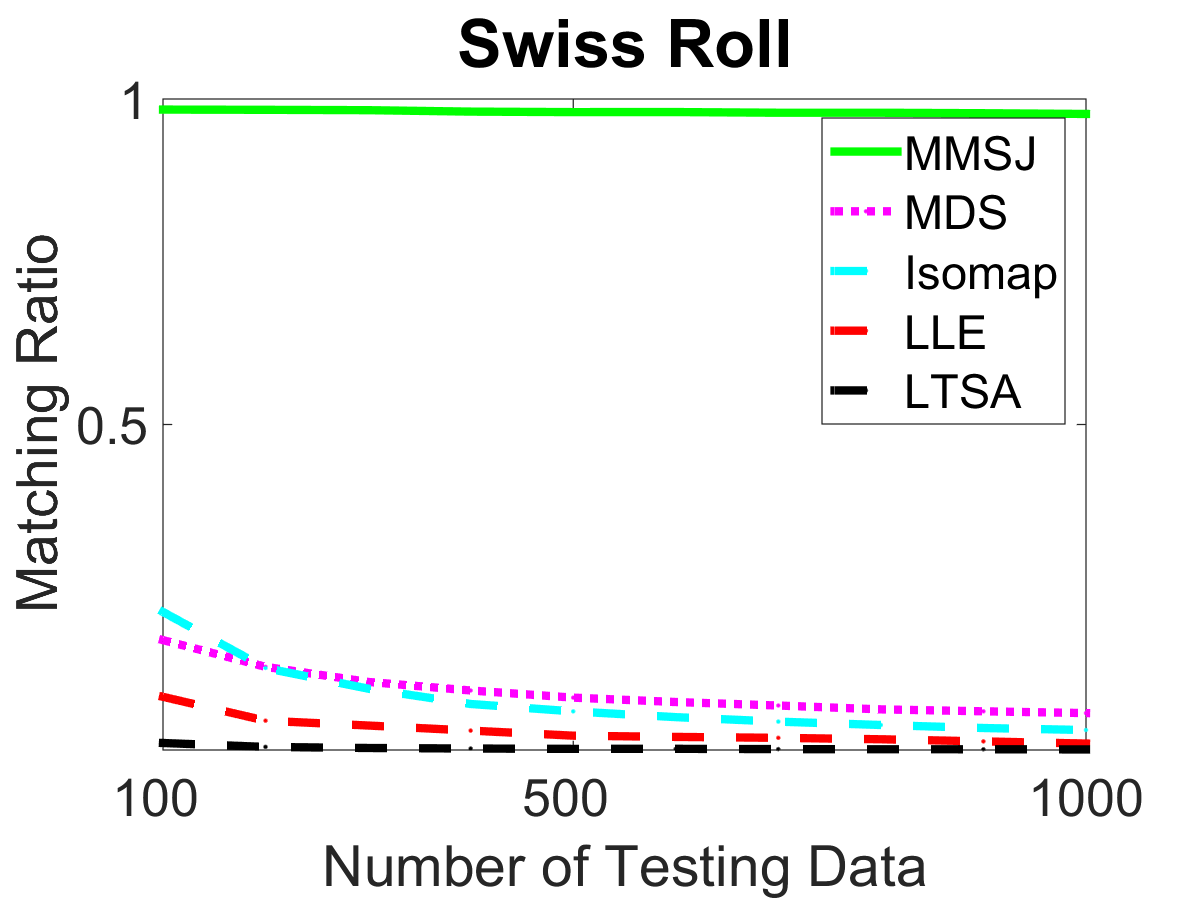
\includegraphics[width=0.5\textwidth]{SwissRollSizeAcc2}
  \caption{ Matching Ratio of 3D Swiss Roll versus its 2D Underlying Linear Manifold via CCA matching, under the same setting as Figure 3. Here the training data is fixed at $n=1000$, while the testing data is allowed to increase from $100$ to $1000$. MMSJ successfully captures the underlying manifolds at $n=1000$, so it is able to maintain an almost perfect matching ratio regardless of the size of the testing data. All other benchmarks have its matching ratio decreasing as the size of the testing data increases, reflecting that the number of the training data is not sufficient for them to fully reveal the underlying manifolds.}
\end{figure*}

%\newpage 

%\section*{Supplementary Material}

\end{document}